%
% lim.tex -- Grenzwert stetiger Funktionen ist unstetig
%
% (c) 2019 Prof Dr Andreas Müller, Hochschule Rapperswil
%
\documentclass[tikz]{standalone}
\usepackage{amsmath}
\usepackage{times}
\usepackage{txfonts}
\usepackage{pgfplots}
\usepackage{csvsimple}
\usetikzlibrary{arrows,intersections,math}
\begin{document}
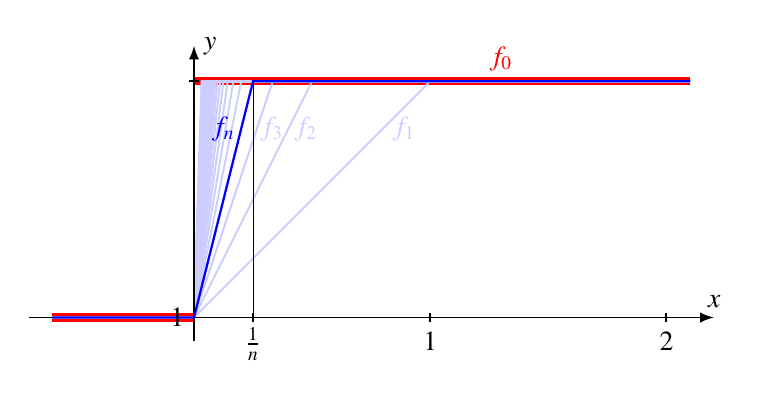
\begin{tikzpicture}[>=latex,scale=3]

\draw[line width=3pt,color=red] (0,1)--(2.1,1);
\draw[line width=3pt,color=red] (-0.6,0)--(0,0);

\foreach \n in {1,...,31}{
	\draw[line width=0.7pt,color=blue!20]
		(-0.6,0)--(0,0)--({1/\n},1)--(2.1,1);
}

\draw[->,line width=0.7pt] (-0.7,0)--(2.2,0) coordinate[label={$x$}];
\draw[->,line width=0.7pt] (0,-0.1)--(0,1.15) coordinate[label={right:$y$}];

\xdef\n{4}
\draw[line width=0.8pt,color=blue] (-0.6,0)--(0,0)--({1/\n},1)--(2.1,1);

\draw[line width=0.1pt] ({1/\n},0)--({1/\n},1);
\draw[line width=0.7pt] ({1/\n},-0.02)--({1/\n},0.02);
\draw[line width=0.7pt] (1,-0.02)--(1,0.02);
\node at (1,-0.02) [below] {$1$};
\draw[line width=0.7pt] (2,-0.02)--(2,0.02);
\node at (2,-0.02) [below] {$2$};
\draw[line width=0.7pt] (-0.02,1)--(0.02,1);
\node (-0.02,1) [left] {$1$};
\node at ({1/\n},0) [below] {$\frac1n$};

\node[color=blue] at ({1/(2*\n)},0.8) {$f_n$};
\node[color=blue!20] at ({0.8*0.3},0.8) [right] {$f_3$};
\node[color=blue!20] at ({0.8*0.48},0.8) [right] {$f_2$};
\node[color=blue!20] at (0.8,0.8) [right] {$f_1$};

\node[color=red] at (1.3,1) [above] {$f_0$};

\end{tikzpicture}
\end{document}

